% % % % % % % % % % % % % % % % % % % % % % % % % % % % % % % % % %
%\documentclass[runningheads]{llncs}
\documentclass[preprint,10pt]{sigplanconf}

% packages
\usepackage{xspace}
\usepackage{ifthen}
\usepackage{amsbsy}
\usepackage{amssymb}
\usepackage{balance}
\usepackage{booktabs}
\usepackage{graphicx}
\usepackage{multirow}
\usepackage{needspace}
\usepackage{microtype}
\usepackage{bold-extra}
\usepackage{array}
\usepackage{epstopdf}


% references
\usepackage[colorlinks]{hyperref}
\usepackage[all]{hypcap}
\setcounter{tocdepth}{2}
\hypersetup{
	colorlinks=true,
	urlcolor=black,
	linkcolor=black,
	citecolor=black,
	plainpages=false,
	bookmarksopen=true}

\def\chapterautorefname{Chapter}
\def\appendixautorefname{Appendix}
\def\sectionautorefname{Section}
\def\subsectionautorefname{Section}
\def\figureautorefname{Figure}
\def\tableautorefname{Table}
\def\listingautorefname{Listing}

% source code
\usepackage{xcolor}
\usepackage{textcomp}
\usepackage{listings}
\definecolor{source}{gray}{0.9}
\lstset{
	language={},
	% characters
	tabsize=3,
	upquote=true,
	escapechar={!},
	keepspaces=true,
	breaklines=true,
	alsoletter={\#:},
	breakautoindent=true,
	columns=fullflexible,
	showstringspaces=false,
	basicstyle=\footnotesize\ttfamily,
	% background
	frame=single,
    framerule=0pt,
	backgroundcolor=\color{source},
	% numbering
	numbersep=5pt,
	numberstyle=\tiny,
	numberfirstline=true,
	% captioning
	captionpos=b,
	% formatting (html)
	moredelim=[is][\textbf]{<b>}{</b>},
	moredelim=[is][\textit]{<i>}{</i>},
	moredelim=[is][\color{red}\uwave]{<u>}{</u>},
	moredelim=[is][\color{red}\sout]{<del>}{</del>},
	moredelim=[is][\color{blue}\underline]{<ins>}{</ins>}}
\newcommand{\ct}{\lstinline[backgroundcolor=\color{white},basicstyle=\footnotesize\ttfamily]}
\newcommand{\lct}[1]{{\small\tt #1}}

% tikz
% \usepackage{tikz}
% \usetikzlibrary{matrix}
% \usetikzlibrary{arrows}
% \usetikzlibrary{external}
% \usetikzlibrary{positioning}
% \usetikzlibrary{shapes.multipart}
% 
% \tikzset{
% 	every picture/.style={semithick},
% 	every text node part/.style={align=center}}
% \tikzexternalize[prefix=figures/]{quality}

% proof-reading
\usepackage{xcolor}
\usepackage[normalem]{ulem}
\newcommand{\ra}{$\rightarrow$}
\newcommand{\ugh}[1]{\textcolor{red}{\uwave{#1}}} % please rephrase
\newcommand{\ins}[1]{\textcolor{blue}{\uline{#1}}} % please insert
\newcommand{\del}[1]{\textcolor{red}{\sout{#1}}} % please delete
\newcommand{\chg}[2]{\textcolor{red}{\sout{#1}}{\ra}\textcolor{blue}{\uline{#2}}} % please change
\newcommand{\chk}[1]{\textcolor{ForestGreen}{#1}} % changed, please check

% comments \nb{label}{color}{text}
\newboolean{showcomments}
\setboolean{showcomments}{true}
\ifthenelse{\boolean{showcomments}}
	{\newcommand{\nb}[3]{
		{\colorbox{#2}{\bfseries\sffamily\scriptsize\textcolor{white}{#1}}}
		{\textcolor{#2}{\sf\small$\blacktriangleright$\textit{#3}$\blacktriangleleft$}}}
	 \newcommand{\version}{\emph{\scriptsize$-$Id$-$}}}
	{\newcommand{\nb}[2]{}
	 \newcommand{\version}{}}
\newcommand{\rev}[2]{\nb{Reviewer #1}{red}{#2}}
\newcommand{\ab}[1]{\nb{Alexandre}{blue}{#1}}
\newcommand{\sv}[1]{\nb{Santiago}{orange}{#1}}

% graphics: \fig{position}{percentage-width}{filename}{caption}
\DeclareGraphicsExtensions{.png,.jpg,.pdf,.eps,.gif}
%\graphicspath{{figures/}}
\newcommand{\fig}[4]{
	\begin{figure}[#1]
		\centering
		\includegraphics[width=#2\textwidth]{#3}
		\caption{\label{fig:#3}#4}
	\end{figure}}
\newcommand{\largefig}[4]{
	\begin{figure*}[#1]
		\centering
		\includegraphics[width=#2\textwidth]{#3}
		\caption{\label{fig:#3}#4}
	\end{figure*}}

% abbreviations
\newcommand{\ie}{\emph{i.e.,}\xspace}
\newcommand{\eg}{\emph{e.g.,}\xspace}
\newcommand{\etc}{\emph{etc.}\xspace}
\newcommand{\etal}{\emph{et al.}\xspace}

% lists
\newenvironment{bullets}[0]
	{\begin{itemize}}
	{\end{itemize}}

\newcommand{\seclabel}[1]{\label{sec:#1}}
\newcommand{\secref}[1]{Section~\ref{sec:#1}\xspace}
\newcommand{\figlabel}[1]{\label{fig:#1}}
\newcommand{\figref}[1]{Figure~\ref{fig:#1}\xspace}

% D O C U M E N T
% % % % % % % % % % % % % % % % % % % % % % % % % % % % % % % % % %
\begin{document}

% T I T L E
% % % % % % % % % % % % % % % % % % % % % % % % % % % % % % % % % %

\title{Extending Mondrian with Interactive HTML Visualisation}

\authorinfo{Santiago Vidal}
	{ISISTAN Research Institute, Faculty of Sciences, UNICEN University, Campus Universitario, Tandil, Buenos Aires, Argentina, Also CONICET}
	{svidal@exa.unicen.edu.ar}
\authorinfo{Alexandre Bergel}
	{PLEIAD Lab, Department of Computer Science (DCC), University of Chile, Santiago, Chile}
	{http://bergel.eu}
\authorinfo{Claudia Marcos} 
	{ISISTAN Research Institute, Faculty of Sciences, UNICEN University, Campus Universitario, Tandil, Buenos Aires, Argentina, Also CIC}
	{cmarcos@exa.unicen.edu.ar}
\authorinfo{Tudor G\^irba} 
	{Software Composition Group, University of Bern, Switzerlan}
	{girba@iam.unibe.ch}


\maketitle

% A B S T R A C T
% % % % % % % % % % % % % % % % % % % % % % % % % % % % % % % % % %

\begin{abstract}
\end{abstract}

%: % % % % % % % % % % % % % % % % % % % % % % % % % % % % % % % % %
\section{Introduction}\seclabel{introduction}

%problem

%solution

%surprising result

%contribution

%\item lesson learnt

%outline
The paper is structured as follows.
%\secref{problem} shows the problem we faced when trying to evolve Mondrian.
%\secref{refactoring} describes the aspect-based solution we adopted.
%\secref{results} presents the impact of our solution on Mondrian.
%\secref{relatedWork} briefly revise the related work.
%\secref{conclusion} concludes.


%: % % % % % % % % % % % % % % % % % % % % % % % % % % % % % % % % %
%\section{Refactoring Mondrian to Enable the Extensions}\seclabel{problem}
%
%Implementation of the visitor pattern instead of the displayOn: methods
%Show some benchmarks. We have they in a mail with the subject bench

\section{Protovis}
Protovis [REF] is a visualization toolkit written in JavaScript that allows the creation of complex and interactive graphics in web-browsers without the need of any plugin. The data to be visualized is defined by means of simple marks such as bars, lines or dots. 

For this definition Protovis makes intesive use of functional programming [REF] through a declarative syntax. For example, to define a bar of \ct{height=100} and \ct{width=20} the following code must be used
\begin{lstlisting} 
new pv.Panel().width(150).height(150)
  .add(pv.Bar)
    .data([100])
    .left(10).bottom(0)
    .width(20).height(function(d) d)
  .root.render();
\end{lstlisting}
where \ct{left} and \ct{bottom} define the panel position \ct{x,y} in which the figure is drawn. 


%: % % % % % % % % % % % % % % % % % % % % % % % % % % % % % % % % %
\section{Generating HTML Files using a Visualization Library}\seclabel{refactoring}

\ab{We need some example. For example, how do you translate ``view nodes: MOShape withAllSubclasses''}
\ab{view shape rectangle height: \#numberOfMethods; width: \#numberOfAttributes. view nodes: MOShape withAllSubclasses}

\ab{Layout? Popup?} \sv{I meant, the layout currently supported is the same than Mondrian. That is, we are copying the x,y position of each figure. Regarding the popup, I dind't use the tooltips provided by Protovis. Instead of that I use a tooltip library, called Tipsy, that support HTML code. }

Given a view generated with Mondrian Easel we want to be able to export it to an HTML file using the Protovis toolkit. In addition of obtaining a similar visualization graph, interaction with it (such as drag and drop) is required. The general scenario of exportation is: 
\begin{enumerate}
\item A user generates a view using Mondrian Easel
\item A user chooses the option "Export as HTML"
\item A file that re-create the view found in Mondrian Easel is generated using Protovis. 
\end{enumerate}

The generation of HTML files with Protovis visualizations in Mondrian involves two main steps: (1) the creation of the dataset that contains information on which to base the graph, and (2) the description of the marks to be drawn. The accomplishment of these steps is described in detail in the next sections. 

\subsection{Generating the Datasets}
The standard way to enter data to Protovis is by mean of a JSON (JavaScript Object Notation) description. Owing to the components to be exported are currently drawn in the Mondrian Easel canvas, the dataset description must be inferred from it. As the canvas data is represented by mean of the \ct{MOGraphElement} hierarchy, the dataset description is created through a Visitor pattern [REF GAMMA] as is shown in Figure \ref{fig:VisitorPattern}.
The JSON structure that we generate is created from the nodes and edges drawn in the canvas. For this reason the structure contains two arrays: nodes and links. The former contain a collection of objects that represent nodes by means of information that allows its correct visualization with Protovis. For example, given the next JSON object a node is specified
\begin{lstlisting} 
{
 nodeID:0, nodeShape:"a MORectangleShape", 
 nodeName:"CharacterSet", 
 nodeWidth:5.0, nodeHeight:18, 
 x:5.0, y:241, 
 nodeFillColor:"#F8F8F8", nodeBorderColor:"#000000", 
 nodeType:"parent"
}
\end{lstlisting}
where \ct{nodeID} is a number that identifies a node uniquely. The variable \ct{nodeShape} indicates the kind of shape that must be drawn (in this case a rectangle).Other possible shapes are, for example, circle, label, or an image. The variable \ct{nodeName} contains the text to be displayed by the tooltip of the node. The size of a shape is indicated by \ct{nodeWidth} and \ct{nodeHeight}. The variables \ct{x} and \ct{y} are used to know the position of the canvas in which the node will be displayed. The fill and border colors of a node are indicated through the variables \ct{nodeFillColor} and \ct{nodeBorderColor}. Finally, the variable \ct{nodeType} indicate if

\begin{figure}
\begin{centering}
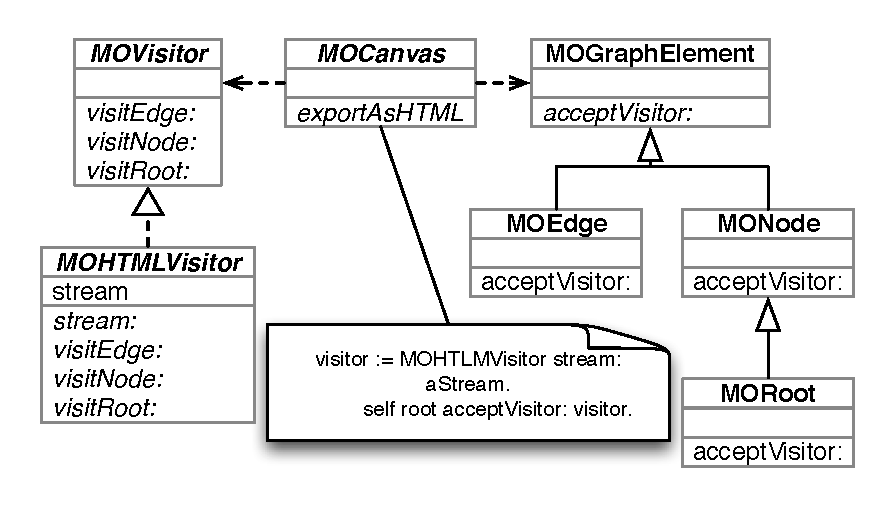
\includegraphics[bb=0bp 0bp 413bp 228bp,scale=0.60]{VisitorPattern} 
\par\end{centering}

\caption{Visitor Pattern.\label{fig:VisitorPattern}}

\end{figure}     
\sv{the examples proposed by Alexandre will be here}
\sv{Explain the implementation of the Visitor pattern that collects the data to generate the HTML file.}

\subsection{Describing the Marks}


\sv{ what are the main benefits of using this kind of visualization.Supported graphs??Layouts.labels and popup.Handling interaction. solving performance issues. Packaging the library files}

%I used the layouts given by Mondrian
%I used Tipsy
%I reimplemented drag&drop
% Some things changed in the drag & drop implementation


Explicar la implementacion con un ejemplo
%: % % % % % % % % % % % % % % % % % % % % % % % % % % % % % % % % %
\section{Future Works}\seclabel{results}
being behind a seaside server


%: % % % % % % % % % % % % % % % % % % % % % % % % % % % % % % % % %
\section{Conclusion}\seclabel{conclusion}



% % % % % % % % % % % % % % % % % % % % % % % % % % % % % % % % % %
%\section*{Acknowledgments}
%
%\small We gratefully thanks ...

% bibliography
% % % % % % % % % % % % % % % % % % % % % % % % % % % % % % % % %
\bibliographystyle{abbrvnat}
\bibliography{}

\end{document}
